\DocumentMetadata{
    pdfversion=1.7,
    pdfstandard=A-3b,
}
\documentclass[11pt,a4paper]{article}

% Set the paper size to A4 with 25 cm margins on all sides
\usepackage[
    a4paper,
    headheight=30pt,
    margin=25mm]{geometry}

%% These three packages together set up STIX fonts 
%% alongside Helvetica
\usepackage[T1]{fontenc}
\usepackage[scaled]{helvet}
\usepackage{stix}           

\usepackage[UKenglish]{babel} % British English conventions
\usepackage[UKenglish,cleanlook]{isodate}   % Date format: day month year

%% For mathematical expresions and units
\usepackage{upgreek}
\usepackage{amsmath}
\usepackage{siunitx}

%% Define variables for the report title and number
\usepackage{xspace}

\makeatletter
\def\reportnumber#1{\gdef\@reportnumber{#1}}
\newcommand{\ReportNumber}{\@reportnumber}
\def\reporttitle#1{\gdef\@reporttitle{#1}}
\newcommand{\ReportTitle}{\@reporttitle}
\newcommand{\ReportReference}{Report No.\xspace \@reportnumber, \@date\xspace}
\newcommand{\LMI}{Lunar Metrology Institute}
\makeatother

%% This package finds the number of pages in a document.
%% The complier must be run twice to find the LastPage number.
\usepackage{lastpage}       
\newcommand{\thispageof}{Page~\thepage~of~\pageref*{LastPage}}

%% Fine control of line spacing 
\usepackage{parskip}        % Paragraph formatting
\usepackage{setspace}

\usepackage{hyperref}
\hypersetup{
    colorlinks=true,        % links are coloured
    urlcolor=blue,          % URLs, etc
    linkcolor=black,        % Pages, etc
    citecolor=blue
}

%% Set up a header and footer
\usepackage{fancyhdr}
 \renewcommand{\headrulewidth}{0pt}  % Supress a line ruled by fancyhdr
 \lhead{
    \fancyplain{} {%
        \small{\centering\textbf{\LMI} \\ 
        \vspace{.5\baselineskip}
        \ReportReference}
    }
 }
 \cfoot{
    \fancyplain{} {%
        \small\textit{This report may not be reproduced, except in full, without the written consent of the\\
        Chief Metrologist, Lunar Metrology Institute}
    }
 }
 \rhead{ \fancyplain{}{\thispageof} }
 \lfoot{}
 \rfoot{}

% A useful reference to the GUM
\newcommand{\referenceGUM}{
For information about uncertainty terminology, see: 
BIPM, IEC, IFCC, ISO, IUPAC, IUPAP and OIML, 
\textit{``Evaluation of measurement data---Guide to the expression of uncertainty in measurement''}, 
BIPM Joint Committee for Guides in Metrology, Paris, S\`evres, edition 1, JCGM~100:2008, 2008. 
A PDF version is available on-line:

\begin{center}
	\href{%
		https://www.bipm.org/documents/20126/2071204/JCGM_100_2008_E.pdf
	}{%
		https://www.bipm.org/documents/20126/2071204/JCGM\_100\_2008\_E.pdf
	}
\end{center}
}

%% These two packages allow the PDF artwork to be loaded
%% in the background for the title page
\usepackage{pdfpages}
\usepackage{eso-pic}
%% A command to produce the title page
\newcommand{\maketitlepage}{%

    % Supress header and footer 
    \thispagestyle{empty}    

    % Page 1 of N is written at the top left
    \thispageof
    
    % A 50 mm vertical space is inserted before writing
    % the report title in a large font size 
    \vspace*{50mm}
    \textbf{\huge \ReportTitle}

    \vspace{5mm}
    \textnormal{\LARGE Thesis Subtitle}
            
    \vspace{1.5cm}
    \textnormal{A thesis presented for the degree of Doctor of Philosophy}\\
    \textnormal{The report number is \ReportNumber}
    
    % Load the background image
    \AddToShipoutPictureBG*{%
        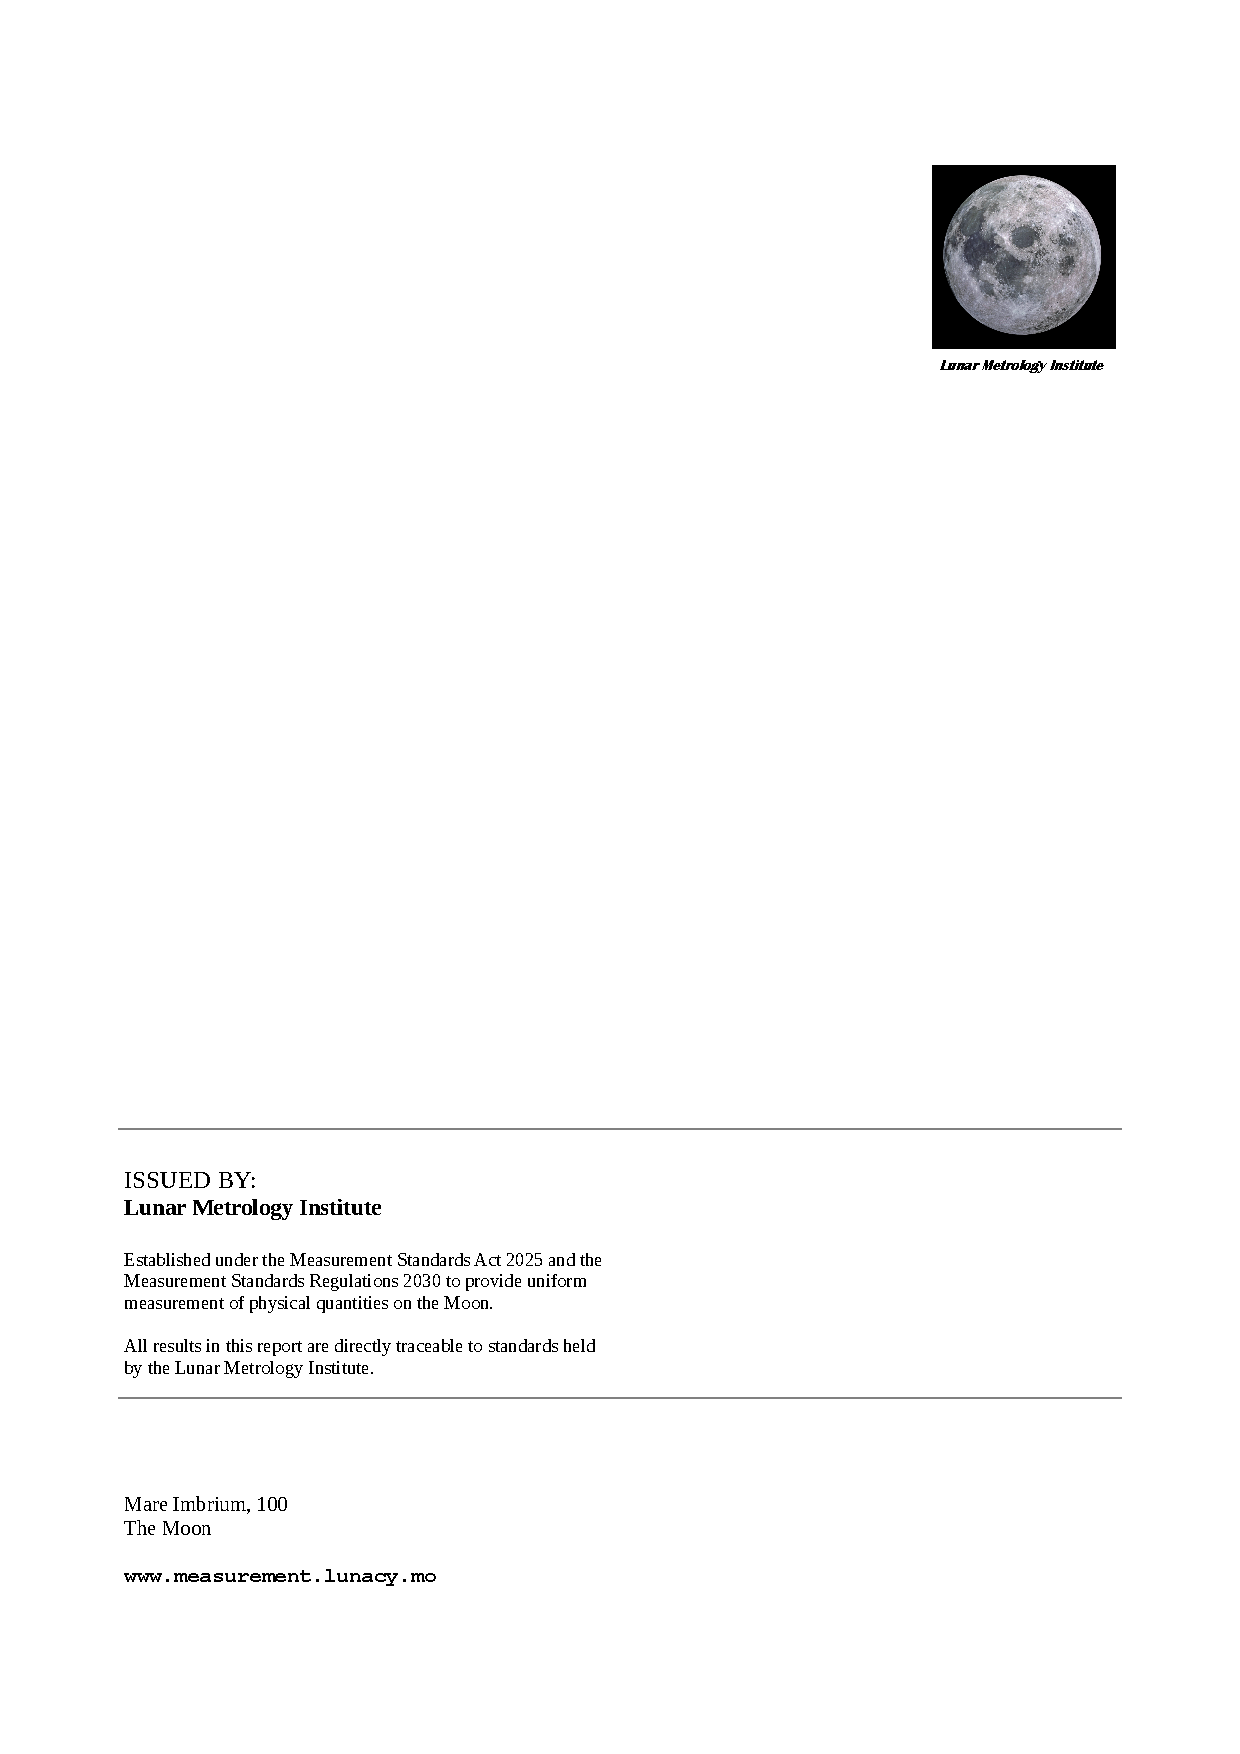
\includegraphics[scale=1]{LMI_cover.pdf}
    }
    % These commands must come after everything else.
    % They insert the background image and signal that 
    % the page is completed. 
    \ClearShipoutPicture
    \clearpage
}
% Fonts!!
% Arial is not in the public domain but Helvetica is very similar.
% So, we use Helvetica (phv).
% The default normal text should be 11-pt. In that case, LaTeX (ref, WikiBooks)
%   \HUGE ~= 23 pt
%   \huge ~= 19 pt
%   \LARGE ~= 16 pt
%   \Large ~= 14 pt
%   \large ~= 12 pt
%   \normal ~= 11 pt
%   \small ~= 10 pt
%   \footnotesize ~= 9 pt
%   \scriptsiize ~= 8.5 pt
%   \tiny ~= 7 pt
%
% The third parameter is the fontseries: `bc` stands for bold condensed
\newcommand{\lmiboldarialnarrow}{\usefont{T1}{phv}{bc}{n}}
\newcommand{\lmiarial}{\usefont{T1}{phv}{m}{n}}
\newcommand{\lmiboldarialsnarrowlanted}{\usefont{T1}{phv}{bc}{sl}}

%% Define the layout of section headings
%% We we would like special fonts and no section numbers 
\usepackage{titlesec}
%% Command formats:
%% \titleformat{<command>}[<shape>]{<format>}
%%      {<label>}{<sep>}{<before-code>}[<after-code>]
%% \titlespacing{<command>}
%%      {<left>}{<before-sep>}{<after-sep>}

\titleformat{\section}
  {\lmiboldarialnarrow\Large}{}{0pt}{}
\titlespacing*{\section}
  {0pt}{\parskip}{0.5\baselineskip} 

\titleformat{\subsection}
    {\lmiboldarialnarrow\large}{}{0.5em}{\vspace{.5em}}
\titlespacing*{\subsection}
    {0pt}{2\parskip}{0.1\baselineskip}

\titleformat{\subsubsection}
    {\lmiboldarialsnarrowlanted\normalsize}{}{0.5em}{\vspace{.25em}}
\titlespacing*{\subsubsection}
    {0pt}{\parskip}{0.1\baselineskip}


%% These details could also come after \begin{document}
\reportnumber{12345} % Usage example
\reporttitle{Thesis Title}
\date{\today}

\begin{document}
\maketitlepage

\pagestyle{fancyplain}
\raggedright        % Does not adjust the right margin
	
% Possible section headings: Description, Identification, Client
% Reference, Date(s) of Calibration (of Test), Objective
% Method, Conditions, Notes, Results, Uncertainty, Conclusion
%
\section{Description}
The components are from a USC vector network analyser calibration kit model 8599. 

\section{Identification}
The component serial number is 2221X.

\section{Client}
United Spacecraft Corporation, 51 Mare Tranquillitatis, The Moon.

\section{Date of Calibration}
The measurements were performed on the 7$^\mathrm{th}$ of February 2025.

\section{Conditions}
Ambient temperature was maintained within $\SI{\pm 1}{\celsius}$ of $\SI{-123}{\celsius}$.

\section{Method}
Measurements of the voltage reflection coefficient were made according to procedure LMIT.E.063.005. 

\section{Results}
Results are reported in polar coordinates (magnitude, $\rho$, and phase, $\phi$), using a linear scale for magnitude and units of degrees for phase. 

% Although not used here, it is also possible to have a \subsubsection{}
\subsection{Open (male), SN 54673}

 \begin{center} % Centered horizontally on the page
 
 % The report text has 1.5 line spacing, 
 % but that is too wide for tables 
 \begin{singlespace}
 
 	\small	% use a smaller font size for the table entries
 
  	% Increases the vertical spacing between rows slightly  
  	\setlength{\extrarowheight}{3pt}
  
	\[
		% the 'S' array column type will align numbers on the decimal 
        % Note 'S[group-minimum-digits=3]' or '\sisetup{group-minimum-digits=3 }'
        % would be used to force a space separator every 3 digits (this
        % does not happen by default until there more than 4 digits)
  		\begin{array}{SSSSS}
    		\multicolumn{1}{c}{ \text{frequency} } & 
    		\multicolumn{2}{c}{ \text{magnitude} } &
    		\multicolumn{2}{c}{ \text{phase} } 
    		\\
		% 2nd line 
    		\multicolumn{1}{c}{ \si{(MHz)} } &  
    		\multicolumn{2}{c}{ (\text{linear}) } &
    		\multicolumn{2}{c}{ \text{(/degree)} }  
    		\\
  		% 3rd line 
     		& {\rho} & {U(\rho)} & {\phi} & {U(\phi)} 
     		\\ \hline % Underline the headings

  		%%-----------------------------------------------
  		% Data here
		45 &   0.9998 &   0.0023$^\dagger$ &    -1.46 &     0.13     \\
		50 &   0.9998 &   0.0023$^\dagger$ &    -1.62 &     0.13     \\
		100 &   0.9999 &   0.0023$^\dagger$ &    -3.27 &     0.13    \\
		300 &   0.9998 &   0.0025 &    -9.80 &     0.14    \\
		500 &   0.9997 &   0.0026 &   -16.34 &     0.15    \\
		1000 &   1.0000 &   0.0032 &   -32.72 &     0.18   \\
		2000 &   0.9994 &   0.0054 &   -65.67 &     0.31  \\
		3000 &    1.000 &    0.011 &   -98.66 &     0.62   \\
		4000 &    0.999 &    0.013 &  -131.74 &     0.78   \\
		5000 &    0.999 &    0.016 &  -164.77 &     0.90   \\
		6000 &    0.998 &    0.017 &  +162.15 &     0.99   \\
		7000 &    0.997 &    0.018 &   +129.0 &      1.1   \\
		8000 &    0.997 &    0.018 &    +95.9 &      1.1   \\
		9000 &    0.996 &    0.018 &    +62.7 &      1.1  \\
		%%-----------------------------------------------
		
		\end{array}
	\]
	
\end{singlespace}
\end{center}


\section{Uncertainty}
A coverage factor $k=1.96$ was used to calculate the expanded uncertainties $U(\cdot)$ at a level of confidence of approximately 95\%. The number of degrees of freedom associated with each measurement result was large enough to justify this coverage factor.  

Some of the expanded uncertainty values reported fall outside LNI's current scope of accreditation. These values are indicated by a $\dagger$. The least expanded uncertainty for a magnitude measurement close to unity in the LNI scope is currently 0.0024. 

% A \paragraph is a lower heirarchy section. The 'heading' text will be in bold
% and the 'body' text will follow on the same line.
\paragraph{Note:} \referenceGUM	% Standard reference to the GUM
\end{document}